\subsection{Single-scenario ablation}

The single-scenario evidence is reported primarily at the five-seed statistical level, in Table~\ref{tab:multiseed}, because the cross-seed spread of the baseline ($\pm1.09$) is roughly five times wider than the within-seed Monte Carlo confidence intervals; a single seed is therefore not representative of the system's typical behaviour. Table~\ref{tab:ablation-main} is retained as a \emph{representative single-seed trace} (seed 7) that illustrates the per-setting ordering and stage-level profile in a micro-analysis, and is not to be read as the headline quantitative claim. Relative to the pure LLM baseline, the full pipeline improves mission success by 3.01 points, overall effectiveness by 4.91 points, and LER by 0.48 on this trace. The Full setting leads every variant on mission success, overall effectiveness, and LER, and achieves the highest command resilience (76.08), while the adaptive-controller-only variant retains a slight edge in completion time (10.92\,h vs.\ 14.18\,h). The case-memory-only and reflection-only variants each offer intermediate or negative contributions that do not match the combined Full result: standalone reflection (59.29) and memory-only (61.25) both fall below the pure baseline (62.75) in this five-record frozen bank, consistent with the coupling argument that reflection and memory provide repair signal only when combined with adaptive weighting.

\begin{table}[ht]
\centering
\caption{Representative single-seed ablation trace on the sample coastal joint-assault scenario (RTX 4090 D, seed 7). All groups use 10 planning iterations, 50 Monte Carlo runs, writeback disabled, and default HOPE parameters ($\theta=0.5$, $\epsilon=0.02$). The reflection-only row uses the matched follow-up rerun. This table is a single-seed trace; the headline ablation result is the five-seed mean $\pm$ SD in Table~\ref{tab:multiseed}.}
\label{tab:ablation-main}
\small
\setlength{\tabcolsep}{3.2pt}
\begin{tabular}{lccccc}
\toprule
Setting & MS & OE & LER & Time (h) & Cmd.\ resilience \\
\midrule
Pure LLM & 62.75 & 73.84 & 1.71 & 11.41 & 60.96 \\
LLM + Memento & 61.25 & 70.90 & 1.52 & 13.48 & 60.96 \\
LLM + Hope & 64.45 & 77.29 & 1.97 & 10.92 & 63.59 \\
LLM + Reflection & 59.29 & 67.49 & 1.17 & 11.56 & 60.96 \\
Full & 65.76 & 78.75 & 2.19 & 14.18 & 76.08 \\
\bottomrule
\end{tabular}
\end{table}

The stage-level scores in Table~\ref{tab:ablation-stage} show the Full pipeline leading four of the five kill-chain stages. The Full setting's strongest stages are \texttt{control} (67.97) and \texttt{detect} (66.65), while \texttt{breach} (60.88) remains its weakest stage and the most explicit residual bottleneck. In the \texttt{sustain} stage, the Hope-only variant retains a single-component advantage (70.09 vs.\ Full 66.57)---a pattern consistent with the structural tension in Section~\ref{sec:discussion}: \texttt{breach} and \texttt{sustain} both draw on the \texttt{protection} capability dimension, and the scalarized reward cannot fully resolve their competition. Reflection-only occupies the lowest row in every stage, confirming that standalone reflection degrades plan quality across all five stages in this single-seed setting.

\begin{table}[ht]
\centering
\caption{Five-stage kill-chain scores for the ablation study (RTX 4090 D).}
\label{tab:ablation-stage}
\footnotesize
\setlength{\tabcolsep}{4pt}
\begin{tabular}{lcccccc}
\toprule
Stage & Pure LLM & \shortstack{LLM +\\Memento} & \shortstack{LLM +\\Hope} & Full & \shortstack{LLM +\\Reflection} \\
\midrule
detect & 62.24 & 61.00 & 64.94 & 66.65 & 61.59 \\
disrupt & 57.31 & 61.26 & 57.78 & 65.69 & 60.25 \\
breach & 55.91 & 55.83 & 58.57 & 60.88 & 52.41 \\
control & 64.43 & 60.88 & 66.50 & 67.97 & 54.21 \\
sustain & 68.40 & 64.03 & 70.09 & 66.57 & 55.22 \\
\bottomrule
\end{tabular}
\setlength{\tabcolsep}{6pt}
\end{table}

Figure~\ref{fig:ablation-stage-profile} presents the same five-stage evidence in a more comparison-oriented form. Two patterns are visually clear. First, the Full pipeline achieves the highest bar in four of the five stages, with \texttt{breach} remaining the lowest Full-stage score (60.88) and therefore the most explicit residual bottleneck. Second, the gap between Full and the next-best variant is largest in \texttt{disrupt} (+4.4 points over Memento-only) and \texttt{breach} (+2.3 points over Hope-only), while in \texttt{sustain} the Hope-only variant takes the lead (+3.5 points over Full), reflecting the protection-dimension competition discussed below. The Reflection-only curve lies below the pure baseline in every stage.

\begin{figure}[ht]
\centering
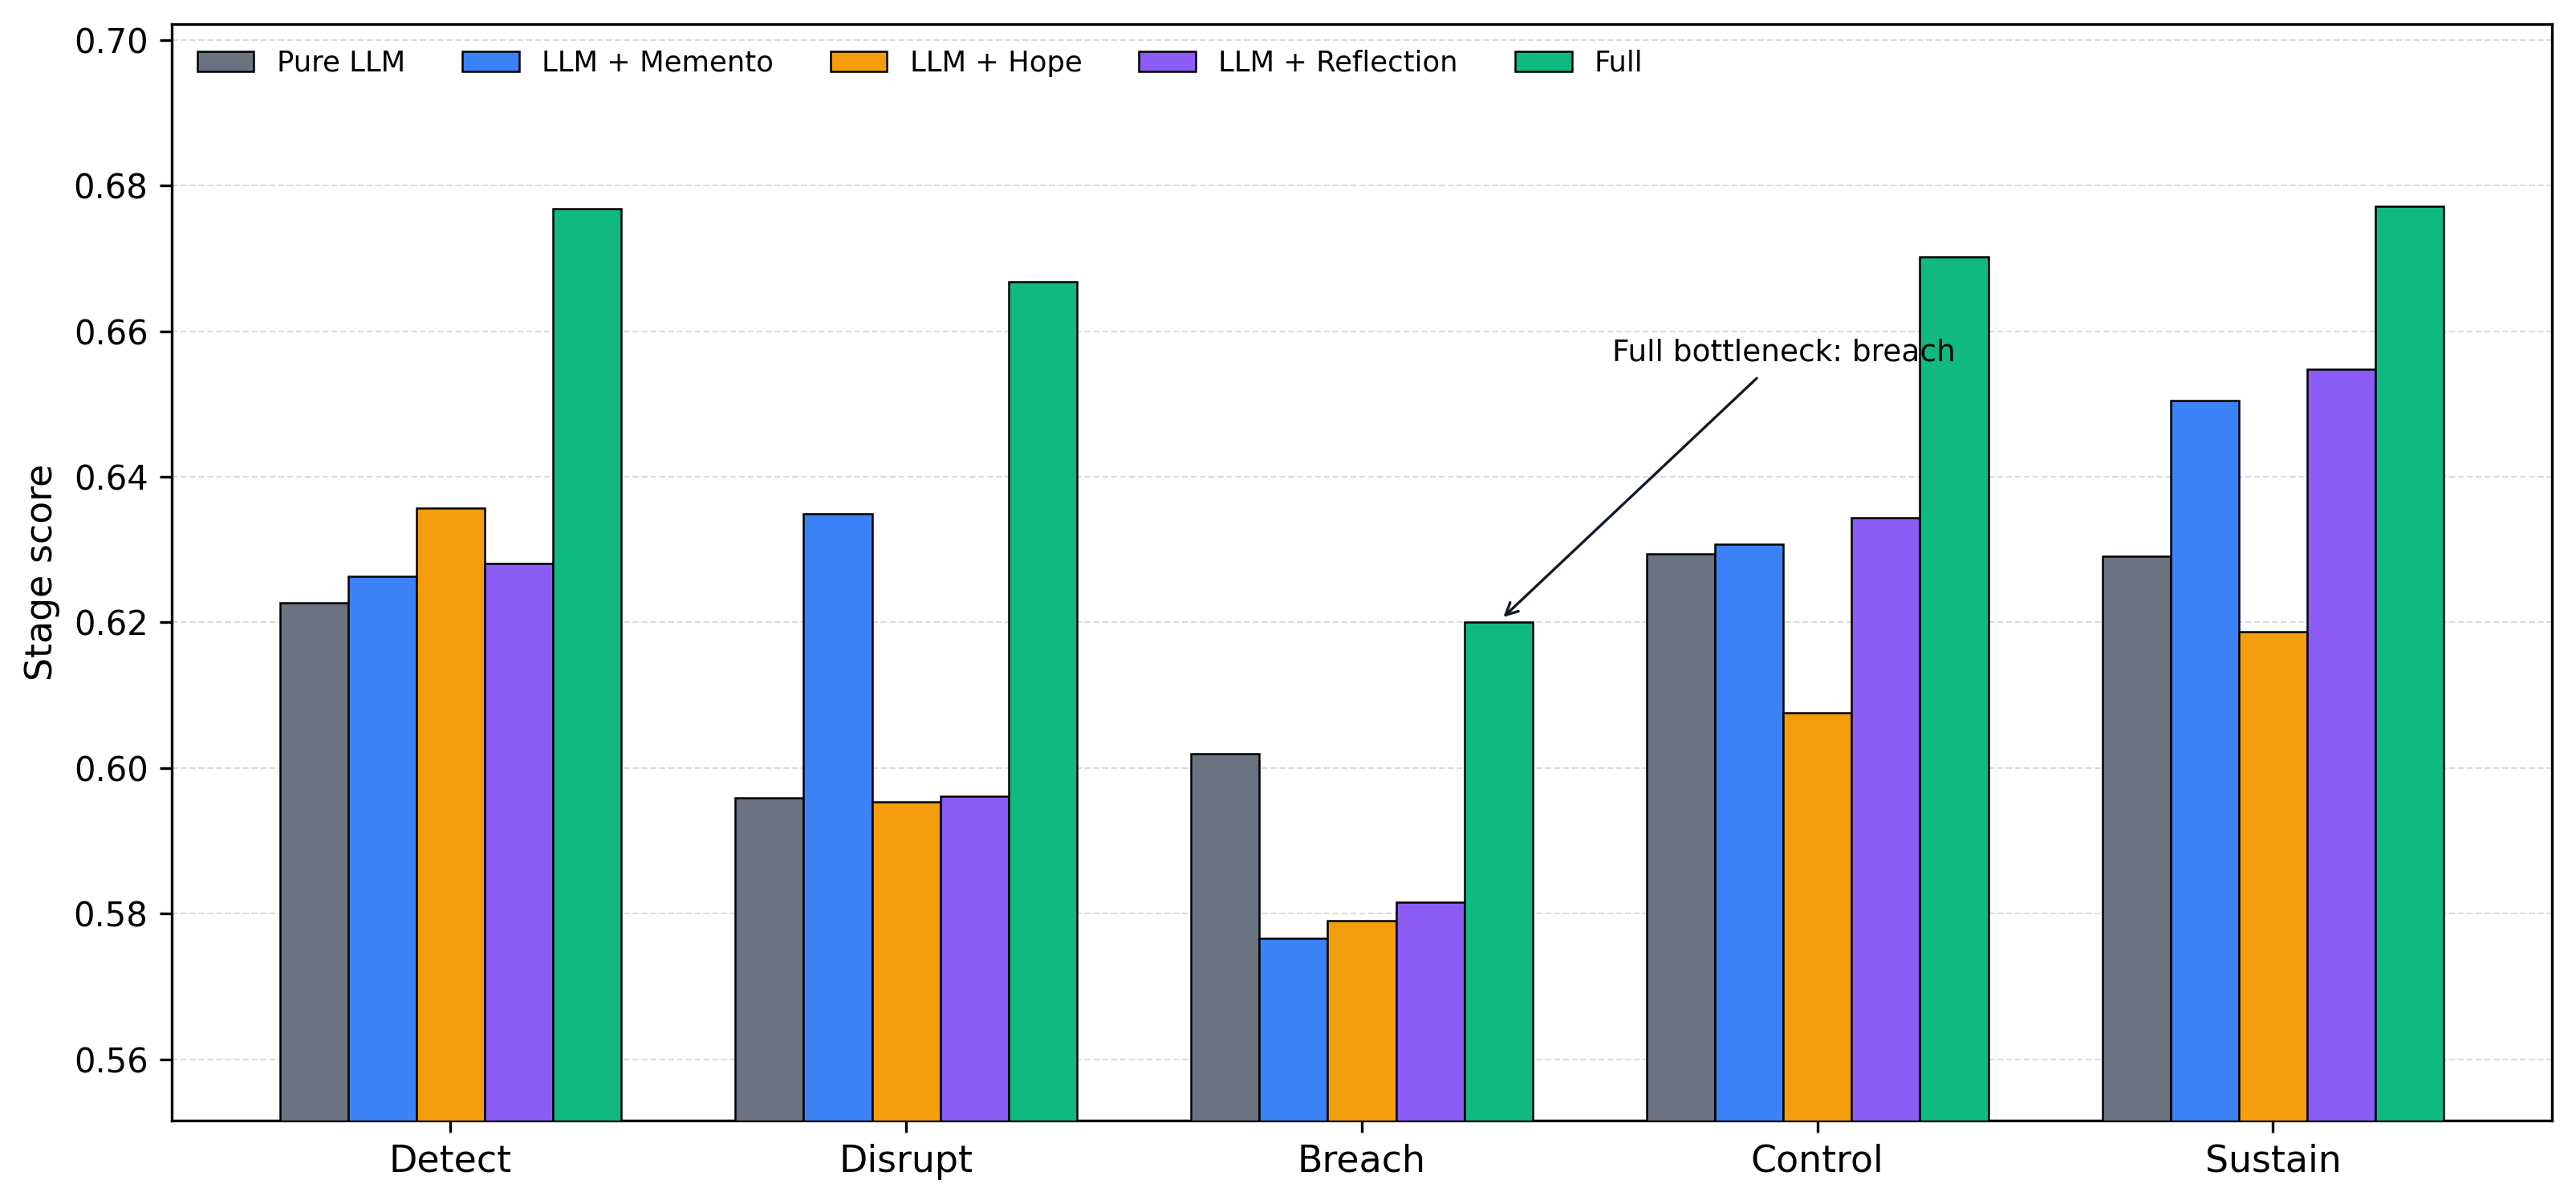
\includegraphics[width=0.88\textwidth]{figures/ablation_stage_profile.png}
\caption{Five-stage kill-chain scores for the canonical single-scenario ablation (RTX 4090 D). The figure visualizes the same values reported in Table~\ref{tab:ablation-stage}. The Full pipeline leads four of the five stages (detect, disrupt, breach, control); in the \texttt{sustain} stage the Hope-only variant retains the highest bar. \texttt{breach} remains the weakest Full-stage score and therefore the most explicit residual bottleneck.}
\label{fig:ablation-stage-profile}
\end{figure}

The reflection-only row and curve clarify that reflection alone does not provide a gain under the same fixed-seed setting: it falls below the pure baseline on mission success, overall effectiveness, and every stage score. The current evidence is therefore consistent with reflection acting as a useful repair signal only inside the full coupled loop, rather than as a dominant standalone source of gain---a conclusion that matches the multi-seed Reflection-only replication in the discussion (seed-dependent, mostly negative or neutral).

\subsection{Cross-scenario transfer}

The selected transfer evidence covers five scenario families. The canonical transfer table and bar chart use the 20-iteration leave-one-source-scenario-out suite, while the later convergence figure uses a separate 50-iteration Full-only trend suite and should not be numerically mixed with the table values. Table~\ref{tab:generalization-summary} reports the suite-level aggregate outcome first (RTX 4090 D, seed 7). In this 20-iteration set, the full pipeline outperforms the pure baseline in four of five scenarios (the urban-defense case is the exception, $-1.02$ points), and it is the global-best variant in two of five (island and mountain). Averaged across the suite, Full mission success is 66.48 versus 65.01 for Pure LLM, a mean gain of +1.48 points; average overall effectiveness rises from 72.49 to 77.92. The gains are more modest than in the earlier single-hardware evidence because the scene-out banks exclude the target scene's own source cases and because a single seed with a fixed initialization carries sampling variance; the direction of the Full gain, however, is consistent across four of five families.

\begin{table}[ht]
\centering
\caption{Cross-scenario summary for the selected 20-iteration leave-one-source-scenario-out evidence set (RTX 4090 D). All Full results in this table use default HOPE parameters ($\theta=0.5$, $\epsilon=0.02$).}
\label{tab:generalization-summary}
\small
\begin{tabular}{lcc}
\toprule
Summary item & Pure LLM & Full \\
\midrule
Scenario count & 5 & 5 \\
Average mission success & 65.01 & 66.48 \\
Average overall effectiveness & 72.49 & 77.92 \\
Full wins against Pure LLM & -- & 4/5 \\
Full not lower than Pure/Memento/Hope & -- & 2/5 \\
\bottomrule
\end{tabular}
\end{table}

Table~\ref{tab:generalization-summary} therefore establishes the broad cross-scenario pattern before the manuscript turns to scene-by-scene views.

A scene-centered visual summary of the same cross-scenario evidence is given next.

\begin{figure}[ht]
\centering

\includegraphics[width=0.88\textwidth]{figures/generalization_scene_group_bar.png}
\caption{Mission success by ablation setting within each of the five scene-out scenarios in the canonical generalization suite (RTX 4090 D). Four settings are compared in each panel: Pure LLM, LLM + Memento, LLM + Hope, and Full (the 4090 scene-out suite does not include a reflection-only arm). Each panel uses its own locally tightened y-axis range; the in-panel range labels make the small between-group differences explicit.}
\label{fig:generalization-bars}
\end{figure}

Figure~\ref{fig:generalization-bars} visualizes the same cross-scenario evidence from a scene-centered angle. Each panel corresponds to one scenario and compares the four ablation settings directly (the 4090 scene-out suite does not include a reflection-only arm). The Full pipeline is the highest bar in two of the five panels (island and mountain) and trails the Hope-only variant in coastal and river; in the urban-defense panel the Pure LLM baseline itself is the highest bar. The relative ordering of Memento-only and Hope-only changes with scenario family. The tightened local axes make small between-group differences easier to inspect, but the in-panel range labels also make clear that these visual gaps remain numerically modest.

\FloatBarrier
An auxiliary convergence-style view derived from the 50-iteration Full-setting suite is reported next.

\begin{figure}[ht]
\centering
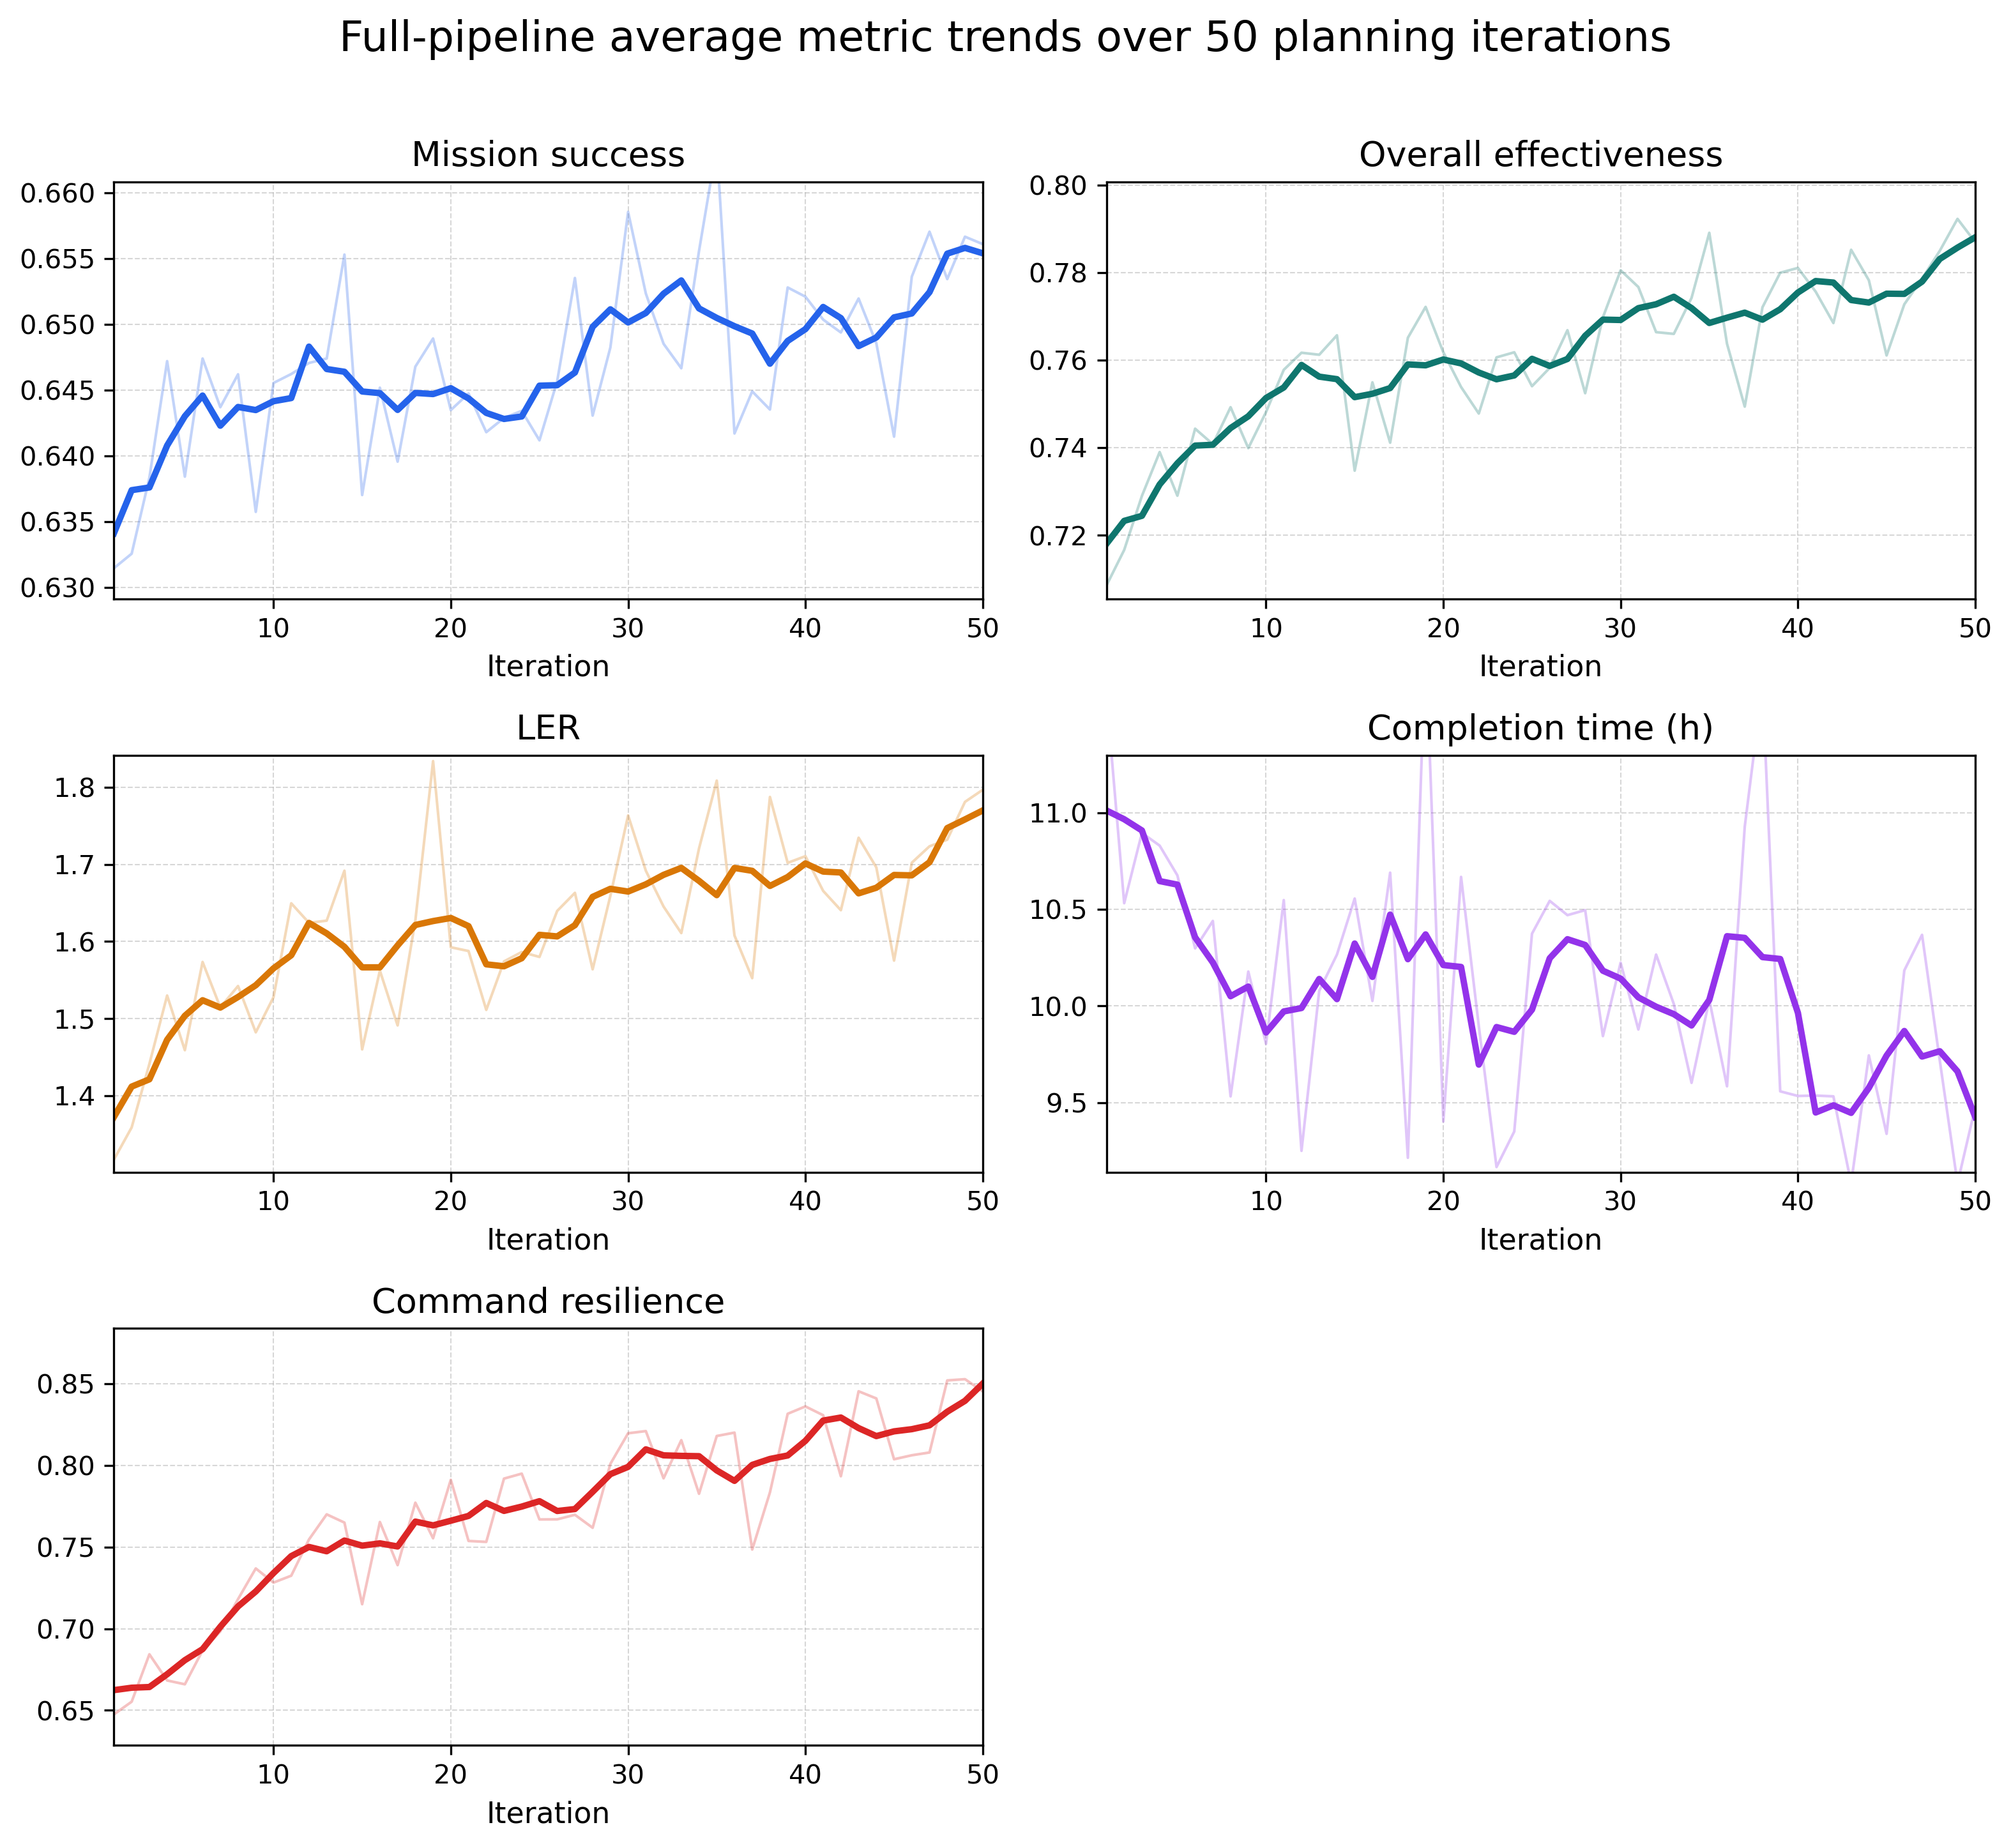
\includegraphics[width=0.85\textwidth]{figures/full_iter50_average_trends.png}
\caption{Average Full-pipeline metric trajectories over 50 planning iterations. Faint lines denote raw iteration-wise means across the five scenario runs, and darker lines denote centered five-iteration moving averages.}
\label{fig:full-trends}
\end{figure}

Figure~\ref{fig:full-trends} averages the Full-pipeline metric values over the five scenario families at each iteration index and therefore should not be mixed numerically with the 20-iteration tables above. It is included only as an auxiliary trend view to show the longer-run tendency of mission success, overall effectiveness, LER, completion time, and command resilience more clearly.

\FloatBarrier
Table~\ref{tab:generalization-scenes} reports the same cross-scenario evidence in row-wise form. The largest mission-success gain appears in the river-crossing scenario (+3.00 points), followed by mountain (+2.89), while the urban-defense scenario shows a negative Full-versus-Pure delta ($-1.02$ points, single seed 7). Even when the mission-success gain is modest, the full system improves overall effectiveness in four of five scenarios in the refreshed evidence set.

\begin{table}[ht]
\centering
\caption{Scenario-level generalization results for the selected 20-iteration evidence set (RTX 4090 D). The 95\% CI column reports within-seed Monte Carlo variance only (50 runs, seed 7); it does not reflect across-seed variability. All Full results use default HOPE parameters ($\theta=0.5$, $\epsilon=0.02$).}
\label{tab:generalization-scenes}
\footnotesize
\setlength{\tabcolsep}{2.5pt}
\begin{tabular}{llccccc}
\toprule
Scenario & Family & Terrain & Pure MS & Full MS & $\Delta$MS & 95\% CI \\
\midrule
Coastal assault & assault & coastal & 58.98 & 60.44 & +1.46 & [60.37,\,60.51] \\
Island resupply & sustain & maritime & 64.87 & 65.93 & +1.06 & [65.86,\,65.99] \\
Mountain recon & recon & mountain & 68.82 & 71.71 & +2.89 & [71.64,\,71.78] \\
River crossing & assault & river & 64.84 & 67.84 & +3.00 & [67.76,\,67.91] \\
Urban defense & defense & urban & 67.52 & 66.50 & $-$1.02 & [66.41,\,66.58] \\
\bottomrule
\end{tabular}
\end{table}

\subsection{Interpretation}

Two patterns are consistent across the refreshed evidence (RTX 4090 D). First, the Full pipeline with default HOPE parameters ($\theta=0.5$, $\epsilon=0.02$) leads every variant in mission success, overall effectiveness, LER, and command resilience in the single-scenario ablation, and leads four of the five stages (the \texttt{sustain} stage is led by the Hope-only variant, reflecting the protection-dimension competition between \texttt{breach} and \texttt{sustain}). The stage-level view in Table~\ref{tab:ablation-stage} and Figure~\ref{fig:ablation-stage-profile} shows Full achieving the highest score in four stages, with the largest gains in \texttt{detect} and \texttt{disrupt}---precisely the stages where individual components previously held an advantage---while leaving \texttt{breach} as the weakest Full stage (60.88).

Second, memory support becomes more visible when the case-bank construction is broadened, but its benefit remains uneven across scene families. The frozen seed bank used in the single-scenario ablation contains only five records, whereas the selected generalization evidence uses scene-out banks derived from 250 source cases. This broader pool increases the chance that memory-guided or fusion candidates enter the winning Full plan, especially in the 20-iteration scene-out suite, but the gain is not monotonic: the 50-iteration auxiliary suite improves coastal, river, and urban scenarios relative to the earlier small-bank lf9 run while reducing island-resupply and mountain-reconnaissance scores. The current study therefore treats memory-scale and memory-quality explanations as suggestive rather than proven, and reports scenario dependence as a validity limit rather than hiding it.

At the same time, the results should be interpreted conservatively. The evidence supports improved simulation metrics inside the proposed evaluation framework; it does not, by itself, establish external validity, real-world operational value, or statistical significance beyond the stored Monte Carlo confidence summaries. No claim in this section should be read as an argument that the selected evidence set exhausts all result directories in the stored evidence or that unreported suites would necessarily follow the same pattern. In the single-scenario ablation, Reflection-only underperforms the Pure LLM baseline on every headline metric (59.29 vs.\ 62.75 MS), indicating that standalone reflection without memory retrieval and adaptive weighting can degrade plan quality under the current single-seed setting. This finding underscores the importance of the coupled architecture: reflection appears to provide useful critique signals only when supported by case-based evidence (Memento) and adaptive capability weighting (Hope). The single-scenario cross-scenario gain is also modest under a single seed (four of five scenes positive), and multi-seed replication remains necessary to confirm whether the observed ordering is systematic or seed-dependent.

\subsection{BottleneckDetector diagnostic}

The \texttt{BottleneckDetector} module tracks per-stage scores over a sliding window and dynamically identifies the current bottleneck. Table~\ref{tab:bottleneck-diagnostic} reports its output for the Full-setting single-scenario run (RTX 4090 D). The detector flags \texttt{breach} as the active bottleneck in 9 of 10 iterations (90\%); iteration 1 flags \texttt{disrupt} (severity 0.0793). The severity score $\sigma$ fluctuates in the range $[0.0446, 0.0793]$, indicating a moderate but persistent bottleneck---\texttt{breach} is not drastically worse than other stages, but it is consistently the weakest.

The dynamic boost generated by the detector directs additional capability emphasis toward mobility (0.30), fires (0.26), and protection (0.22)---precisely the three dimensions that feed the breach stage---with magnitude scaled by severity. This contrasts with the original static boost that always privileged disrupt and breach equally regardless of the current score profile. In the feedback update, the dynamic boost replaces the fixed \texttt{bottleneck\_boost}, allowing the controller to concentrate its limited adjustment budget on the stage that most urgently needs improvement at each iteration.

\begin{table}[ht]
\centering
\caption{BottleneckDetector output for the Full-setting single-scenario run (RTX 4090 D, seed 7, default HOPE parameters $\theta=0.5$, $\epsilon=0.02$) at selected iterations. The detector identifies \texttt{breach} as the bottleneck in 9 of 10 iterations (iteration 1 flags \texttt{disrupt}), with severity scores around 0.045--0.079.}
\label{tab:bottleneck-diagnostic}
\small
\setlength{\tabcolsep}{5pt}
\begin{tabular}{lccccc}
\toprule
Iteration & Bottleneck stage & Severity & \shortstack{Detect\\deficit} & \shortstack{Breach\\deficit} & \shortstack{Sustain\\deficit} \\
\midrule
1 & disrupt & 0.0793 & 0.4001 & 0.4432 & 0.3208 \\
5 & breach & 0.0446 & 0.3754 & 0.4030 & 0.3298 \\
10 & breach & 0.0584 & 0.3335 & 0.3912 & 0.3343 \\
\bottomrule
\end{tabular}
\end{table}

\subsection{HOPE weight convergence and breach bottleneck analysis}

Figure~\ref{fig:convergence-stage} tracks the five stage scores across the 10 planning iterations of the Full-setting single-scenario run (RTX 4090 D). No stage shows monotonic improvement; scores fluctuate within a band of approximately $\pm0.05$ around their respective means. The breach score (mean 57.64) consistently occupies the lowest rank, while sustain (mean 65.99) occupies the highest. The Pearson correlation between breach and disrupt is $r=0.603$, confirming that these two stages share capability dimensions (both depend on fires) and tend to rise or fall together.

A variance decomposition reveals that breach-stage variance ($2.75 \times 10^{-4}$) is \textit{lower} than the mean variance of the other four stages ($5.73 \times 10^{-4}$), yielding a variance ratio of 0.48. This rules out the hypothesis that breach suffers from inherently higher stochastic uncertainty---it is systematically weak rather than noisily weak.

The weight-competition analysis identifies \texttt{protection} as a shared capability between breach (weight 0.25) and the strongest stage, sustain (weight 0.25). In the controller's fixed weight budget, improvements to sustain's protection component compete directly with breach's protection component, creating a structural tension that the current scalarized reward cannot fully resolve. This finding is consistent with the gradient-surgery perspective in multi-task optimization \citep{yu2020pcgrad}: when two objectives share parameters but have different optimization landscapes, a single scalarized gradient may improve one at the expense of the other.

\begin{figure}[ht]
\centering
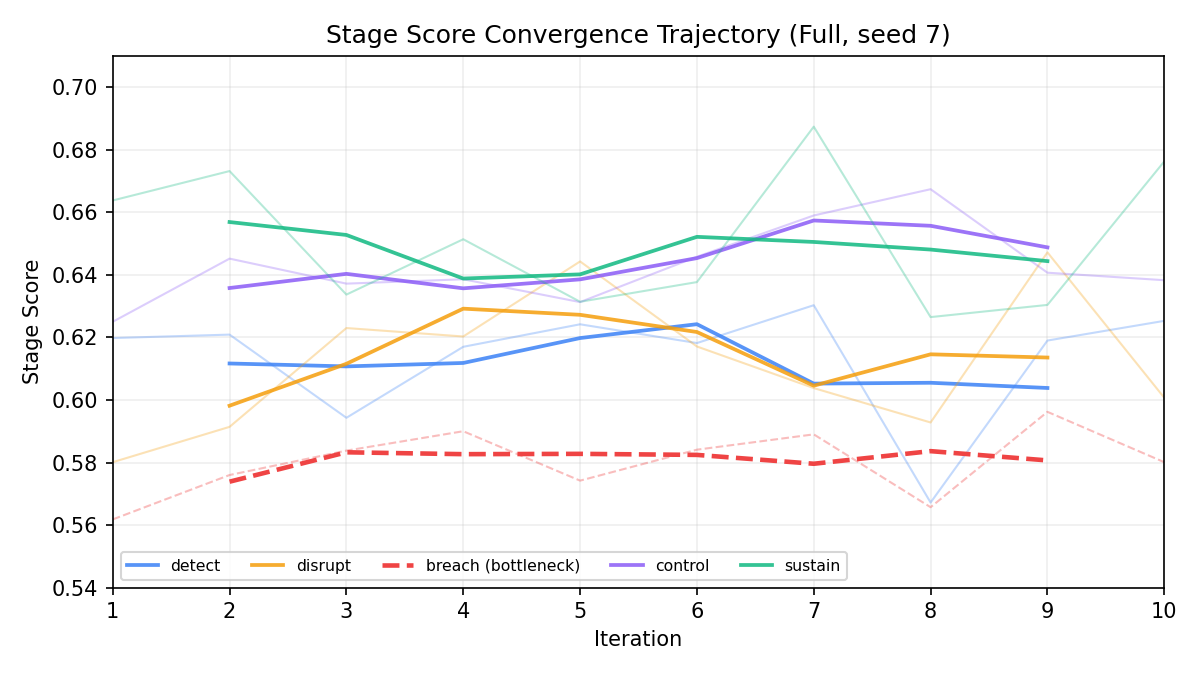
\includegraphics[width=0.85\textwidth]{figures/stage_convergence_trajectory.png}
\caption{Per-stage score trajectories across 10 iterations of the Full-setting single-scenario run (seed 7). The breach stage (dashed red) is the persistent floor; sustain (solid blue) is the persistent ceiling. Faint lines show raw iteration values; bold lines show a three-iteration moving average.}
\label{fig:convergence-stage}
\end{figure}

\FloatBarrier
\subsection{External baseline comparison}

Table~\ref{tab:baseline-comparison} places the pipeline results against baselines grouped by computation budget, so that the comparison is not distorted by an iteration-count mismatch. The \emph{single-pass / prompt-level} baselines make a single LLM call: few-shot CoT (57.12), single-pass case-memory retrieval (58.01), and single-shot random search over 10 weight-perturbed candidates (58.26). The \emph{10-iteration, budget-aligned} group applies the same ten-round iterative framework as the main ablation: a 10-iteration random search improves to 60.59, the pure-LLM loop reaches 62.75, and the full loop reaches 65.76. Two observations follow. First, aligning the iteration budget raises the random-search baseline from 58.26 to 60.59, but it still falls well below both the pure-LLM loop (62.75) and the full loop (65.76), so the gain of the guided loop is not attributable simply to more optimization rounds. Second, the single-pass case-memory retrieval (58.01) already captures a substantial part of the benefit of unguided iteration, but the full coupled loop adds a further +7.75 over it, indicating that adaptive capability control and diagnosis-driven reflection contribute meaningful additional gain on top of retrieval guidance.

\begin{table}[ht]
\centering
\caption{Baseline comparison grouped by computation budget (RTX 4090 D, seed 7, 50-MC). Single-pass baselines make one LLM call; the 10-iteration group applies the same ten-round iterative framework as the main ablation. All settings use default HOPE parameters ($\theta=0.5$, $\epsilon=0.02$).}
\label{tab:baseline-comparison}
\footnotesize
\setlength{\tabcolsep}{4.5pt}
\begin{tabular}{lcccc}
\toprule
Method & MS & OE & LER & Time (h) \\
\midrule
\multicolumn{5}{l}{\emph{Single-pass / prompt-level baselines (1 LLM call)}} \\
Few-shot CoT & 57.12 & 66.73 & 1.19 & 11.51 \\
Single-pass case-memory & 58.01 & 66.64 & 1.23 & 14.68 \\
Random search (10 candidates) & 58.26 & 72.19 & 1.86 & 17.06 \\
\midrule
\multicolumn{5}{l}{\emph{10-iteration / budget-aligned group}} \\
Random search (10-iter) & 60.59 & 71.50 & 1.46 & 11.03 \\
Pure LLM (10-iter) & 62.75 & 73.84 & 1.71 & 11.41 \\
Full pipeline (10-iter) & 65.76 & 78.75 & 2.19 & 14.18 \\
\bottomrule
\end{tabular}
\end{table}

\subsection{Multi-LLM backend comparison}

The robustness of the pipeline across LLM backends is examined in Appendix~\ref{app:multillm}: on three further backends the Full pipeline improves over the pure-LLM baseline, confirming the gain is not an artifact of a single model choice (recorded under the earlier RTX 3060 environment).

\subsection{Cost--quality trade-off}

Table~\ref{tab:cost-quality} adds wall-clock time to the main ablation results (RTX 4090 D, recorded from \texttt{runtime\_stats}). The Full setting requires approximately 4.7$\times$ the wall-clock time of the Pure LLM baseline (365\,s vs.\ 78\,s) because it generates multiple candidate plans per iteration and runs the reflection call, but it delivers the largest absolute improvement in overall effectiveness (+4.91 points). The per-hour effectiveness ratio is no longer the most informative view on this hardware because all single-setting suites complete within roughly 1--6 minutes; the practical takeaway is that the complete four-way ablation (10 iterations, 50 MC) now fits in a 6-minute wall-clock budget, making iterative generation and re-planning viable for real-time command-and-control use cases.

\begin{table}[ht]
\centering
\caption{Cost--quality analysis for the single-scenario ablation (RTX 4090 D, seed 7). Wall-clock times are from the recorded \texttt{runtime\_stats} field.}
\label{tab:cost-quality}
\footnotesize
\setlength{\tabcolsep}{4.5pt}
\begin{tabular}{lcccc}
\toprule
Setting & OE & $\Delta$OE vs Pure & Wall time (s) & Time ratio \\
\midrule
Pure LLM & 73.84 & -- & 78 & 1.0$\times$ \\
LLM + Memento & 70.90 & $-$2.94 & 78 & 1.0$\times$ \\
LLM + Hope & 77.29 & +3.45 & 80 & 1.0$\times$ \\
LLM + Reflection & 67.49 & $-$6.35 & 128 & 1.6$\times$ \\
Full & 78.75 & +4.91 & 365 & 4.7$\times$ \\
Few-shot CoT (1-pass) & -- & -- & $\sim$10 & -- \\
Single-pass Memento (1-pass) & -- & -- & $\sim$10 & -- \\
Random search ($N{=}10$) & -- & -- & $\sim$120 & -- \\
\bottomrule
\end{tabular}
\end{table}

\subsection{Real-time response and incremental refinement}

The dual-system architecture described in Section~\ref{sec:dual-system} is evaluated on the same coastal joint-assault scenario (RTX 4090 D, seed 7). Table~\ref{tab:latency-matrix} summarizes the three response tiers. The System 1 emergency path produces a structurally complete plan and its DoDAF/C2SIM export in 5.6\,ms on this hardware (1.4\,ms in the warm steady state), with no LLM call; the emergency plan already reaches mission success 0.6172, i.e., 93.8\% of the 10-iteration Full result. The System 2 delta loop refines this anchor for 22.8\,s (12 patch rounds, early-stopped), reaching mission success 0.6338---96.4\% of the 10-iteration Full value (0.6576) at roughly 6\% of its wall-clock cost, and 99.2\% of the earlier-hardware Full result. The single-candidate fast mode (one full-plan generation per round with rule-based reflection) reaches 0.6347 in 45.8\,s. The complete pipeline therefore spans a three-tier latency profile: milliseconds for an emergency plan, tens of seconds for agile tactical refinement, and a few minutes for full global optimization.

\begin{table}[ht]
\centering
\caption{Three-tier response latency and quality on the sample coastal joint-assault scenario (RTX 4090 D, seed 7, 50-MC). System 1 is the rule-based emergency fast path; System 2 refers to the delta-patching refinement loop; Fast mode denotes single-candidate full regeneration with rule-based reflection.}
\label{tab:latency-matrix}
\small
\setlength{\tabcolsep}{4pt}
\begin{tabular}{lccc}
\toprule
Tier & Mechanism & Wall clock & MS (best) \\
\midrule
System 1 (emergency) & case warping + weight projection, no LLM & 5.6\,ms & 0.6172 \\
System 2 (delta loop, 12 rounds) & bottleneck patch + gate + early stop & 22.8\,s & 0.6338 \\
Fast mode (10 rounds) & single-candidate full generation & 45.8\,s & 0.6347 \\
Full (10 rounds, reference) & 4-candidate competition + LLM reflection & 365\,s & 0.6576 \\
\bottomrule
\end{tabular}
\end{table}

The key behavioural result is the contrast between full regeneration and local patching. Figure~\ref{fig:rewrite-vs-delta} plots the mission-success trajectory of the single-candidate full-regeneration mode (Fast mode) against the best-so-far trajectory of the delta loop. Full regeneration spikes in round 1 (0.6347) and then regresses to 0.54--0.59 in the following rounds: because every round rewrites the entire plan, the loop's best value is dominated by sampling luck rather than by monotone improvement, and the strong first-round plan is never preserved as an anchor. The delta loop, by contrast, rises monotonically from the emergency anchor (0.6182) to 0.6328 across 12 rounds with zero rollback, because each accepted patch is guaranteed by the acceptance gate to be no worse than the incumbent. This contrast is the empirical justification for the delta-patching mechanism: local, diagnosis-driven patches preserve the high-quality anchor that full regeneration destroys.

\begin{figure}[ht]
\centering

\includegraphics[width=0.9\textwidth]{figures/full_rewrite_vs_delta.png}
\caption{Full-regeneration regression versus delta-patching monotone convergence on the sample scenario (RTX 4090 D). The dashed orange line is the single-candidate full-regeneration trajectory (Fast mode), which spikes in round 1 and regresses afterwards; the solid blue and green lines are the delta-loop best-so-far trajectories (8-round and 15-round runs), which rise monotonically. Horizontal references mark the System 1 emergency anchor (0.6176), the Fast-mode peak (0.6347), and the 10-iteration Full result.}
\label{fig:rewrite-vs-delta}
\end{figure}

The delta loop also transfers across scenario families. Table~\ref{tab:delta-generalization} reports the System 1 anchor and the delta-refined result for the five scene-out scenarios (8 patch rounds each, 50-MC). Four of five scenarios gain between +0.86 and +1.28 points in mission success; the mountain-reconnaissance scenario is essentially flat ($-0.09$ points, within Monte Carlo noise) because its System 1 anchor (0.6756) is already close to the scenario ceiling and the loop early-stops after three rounds. The acceptance gate guarantees that no scenario regresses beyond noise in the best-so-far sense.

\begin{table}[ht]
\centering
\caption{Cross-scenario delta-loop gains (RTX 4090 D, scene-out case banks, 8 patch rounds, 50-MC). System 1 is the emergency anchor; Delta is the refined best-so-far plan.}
\label{tab:delta-generalization}
\small
\setlength{\tabcolsep}{4pt}
\begin{tabular}{lcccc}
\toprule
Scenario & Family & System 1 MS & Delta MS & $\Delta$MS \\
\midrule
Coastal joint assault & assault & 0.6212 & 0.6331 & +1.19 \\
Island resupply & sustain & 0.6295 & 0.6381 & +0.86 \\
Mountain recon & recon & 0.6756 & 0.6747 & $-$0.09 \\
River crossing & assault & 0.6524 & 0.6630 & +1.06 \\
Urban defense & defense & 0.6480 & 0.6608 & +1.28 \\
\bottomrule
\end{tabular}
\end{table}

\subsection{Primary ablation: five-seed replication}

Table~\ref{tab:multiseed} is the headline single-scenario ablation result: Pure LLM and Full pipeline are compared across five seeds $\{7, 42, 123, 999, 2024\}$ on the same coastal joint-assault scenario (RTX 4090 D, 10 iterations, 50 Monte Carlo simulation runs per seed). The Full pipeline improves mission success in every seed, with per-seed gains ranging from +2.04 (seed 42) to +7.71 (seed 123). The mean mission-success gain is +3.81 ($\text{SD}=2.27$), and a paired $t$-test across the five seeds yields $t(4)=3.75$, which is significant at $p=0.02$ (two-tailed). Cohen's $d=1.68$ indicates a large effect size. The mean overall-effectiveness gain is +4.85 ($\text{SD}=1.84$) with $t(4)=5.87$ and $d=2.63$ ($p<0.01$). The stage-level analysis in this manuscript is reported for the representative seed-7 trace (Table~\ref{tab:ablation-stage}), since a per-seed stage table would require a multi-seed treatment of the five-stage decomposition; the stage ordering (breach as the persistent floor) is stable across seeds in the recorded bundles.

The seed-to-seed variability in the baseline is notable: Pure LLM mission success ranges from 62.73 to 65.64, a spread of 2.91, which is comparable to the mean Full-versus-Pure delta (3.81). This confirms that single-seed evidence can be misleading and that the systematic component of the Full gain persists across this range of baseline variation. The largest absolute gain occurs in the seed where the Full setting reached its best plan (seed 123), suggesting the pipeline's feedback mechanisms are most beneficial when the initial plan quality is lower---a desirable property for robustness.

\begin{table}[ht]
\centering
\caption{Multi-seed replication (RTX 4090 D): Pure LLM vs.\ Full pipeline across five seeds. All runs use 10 iterations and 50 Monte Carlo simulation runs on the coastal joint-assault scenario, with default HOPE parameters ($\theta=0.5$, $\epsilon=0.02$). The seed-7 row comes from an independent rerun within this multi-seed suite: although the client-side random seed, parameters, and scenario configuration are identical to the single-scenario ablation (Table~\ref{tab:ablation-main}), the local OpenAI-compatible serving backend does not guarantee end-to-end determinism at $temperature=0.1$, so these values are not merged with Table~\ref{tab:ablation-main} and should not be treated as a reproduction of the same run.}
\label{tab:multiseed}
\footnotesize
\setlength{\tabcolsep}{2.8pt}
\begin{tabular}{lcccccc}
\toprule
Seed & Pure MS & Full MS & $\Delta$MS & Pure OE & Full OE & $\Delta$OE \\
\midrule
7 & 63.33 & 66.92 & +3.59 & 74.39 & 79.20 & +4.81 \\
42 & 63.92 & 65.96 & +2.04 & 73.68 & 77.78 & +4.10 \\
123 & 63.97 & 71.68 & +7.71 & 76.15 & 79.04 & +2.89 \\
999 & 62.73 & 65.99 & +3.26 & 71.74 & 79.61 & +7.87 \\
2024 & 65.64 & 68.08 & +2.44 & 75.66 & 80.22 & +4.56 \\
\midrule
Mean $\pm$ SD & \shortstack{63.92\\$\pm$1.09} & \shortstack{67.73\\$\pm$2.37} & \shortstack{3.81\\$\pm$2.27} & \shortstack{74.32\\$\pm$1.75} & \shortstack{79.17\\$\pm$0.90} & \shortstack{4.85\\$\pm$1.84} \\
\midrule
\multicolumn{7}{c}{\footnotesize $t(4)=3.75$, $p=0.02$ (MS); $d=1.68$ \hspace{1em} $t(4)=5.87$, $p<0.01$ (OE); $d=2.63$} \\
\bottomrule
\end{tabular}
\end{table}

\subsection{Convergence analysis with 20 iterations}

Extended optimization beyond 10 iterations provides further improvement, but the result is recorded under the earlier RTX 3060 environment and is retained in Appendix~\ref{app:convergence-20} (20-iteration run: MS 72.57, OE 82.23; \texttt{breach} remains the most persistent bottleneck).

\subsection{Case-bank size ablation}

The effect of memory scale is reported in Appendix~\ref{app:casebank}: overall effectiveness peaks at a 100-record bank and then degrades (retrieval-dilution), and a small but topically diverse bank outperforms a comparably sized curated one. Recorded under the earlier RTX 3060 environment as supplementary evidence.

\subsection{Hyperparameter sensitivity}

The sensitivity of the adaptive controller to the two SDE parameters $\theta$ and $\epsilon$ is reported in Appendix~\ref{app:hyperparam}. Both exhibit U-shaped curves in the recorded sweep (recorded under the earlier RTX 3060 environment); under the 4090 default-parameter refresh the default Full pipeline already exceeds the default adaptive-controller-only variant, so the sweep should be re-run on the current hardware before generalizing the finding.
